
%\chapter{In-progress - A deeper exploration of potentiation in associative learning}
%\chapter{Twisting Fates: Individual Mutations Potentiate the Evolution of Associative Learning}
% Evolutionary Catalysts 
% Recognizing Potential: Identiying individual mutations that catalize evolutionary outcomes.
% On the Ubiquitousness of Potentiating Mutations (in Avida)
%\chapter{The ubiquitous potentiating mutation: A large-scale study of associative learning in Avida}
%\chapter{The ubiquity of potentiating mutations: A large-scale study of historical contingency in Avida}
\chapter{A large-scale digital evolution study of historical contingencies in associative learning}

\label{chap:learning_distributions}

\noindent
Authors: Austin J. Ferguson and Charles Ofria 

\noindent This chapter is in final preparation before submission.

This chapter directly extends the previous chapter. 
We expand from analyzing the potentiation dynamics of four case study lineages to replaying 50 lineages.
With this larger dataset, we begin to conduct statistically powerful analyses of the the distribution of potentiation changes. 
In all 50 lineages we find a single-generation step in the lineage where the potentiation of associative learning increases significantly. 
Further, we verify that these increases are most often driven by a single mutation, though we do find evidence that multiple mutations can interact to increase potentiation. 
We find that these large potentiation increases are comparable to some, but not all, previous works on potentiation, and discuss those comparisons in detail. 


% \noindent
% Authors: Austin Ferguson and Charles Ofria

% \noindent
% Status: This is a direct extension of Chapter \ref{chap:alife_submission}.
% It is marked in-progress as all software has been implemented and additional explorations beyond Chapter \ref{chap:alife_submission} have been conducted to identify useful changes to parameters and the environment. 
% The actual data collection, however, has yet to begin. 
% Note that this chapter may make Chapter \ref{chap:alife_submission} redundant in the final dissertation.
% Both are included here, however, as Chapter \ref{chap:alife_submission} serves as preliminary results for this chapter. 

% Introduction
% Succinct, with no subheadings.

% What events were \textit{key} in the fall of an empire? 
% What turns solidified your victory in that board game? 
% What mutations were most important in the evolution of that behavior? 
% Alas, while these are all valid questions, the sheer number of possibilities means that we will likely never know the answers. 
% That is, unless we are talking about digital evolution, in which we have reached a point where it is computationally feasible to decypher which mutations had the largest effect on the final evolved population. 

%In the natural world, we typically see the fruits of evolution's labor. 
%Even in experimental evolution, we only see

\section{Introduction}

In Chapter \ref{chap:learning_case_studies} I conducted four case studies and analyzed the genetic potentiation of associative learning in the Avida digital evolution system. 
As in the previous chapter, here I use ``genetic potentiation'' to refer to changes in the genetic background that promote the evolution of a particular trait or behavior, in this case associative learning \citep{blountHistoricalContingencyEvolution2008}.
%In the previous chapter, 
We found that potentiation can increase over a short period of time, including a single mutation between parent and offspring. 
While I conducted a deep examination of the observed potentiation dynamics in Chapter \ref{chap:learning_case_studies}, I limited myself to examining only four case study lineages. 
Here, I expand this work by again replaying the evolution of associative learning in Avida, but shifting from detailed case studies to aggregate data by analyzing the potentiation dynamics of 50 lineages. 

My overall goal for this work is to provide a more comprehensive point of comparison for other studies on potentiation dynamics. 
While several previous studies of potentiation dynamics exist, they all analyze the dynamics of only one or at most a few lineages.
By analyzing 50 lineages, here we shift from a few data points of potentiation measurements to full distributions backed by statistically powerful conclusions. %will not have a few data points for particular potentiation measurements, but rather distribution estimates. 
With this work, I aim to accomplish two goals: 
1) to allow us to examine previous studies in a new light, possibly identifying trends in potentiation dynamics across systems, and 
2) to provide a benchmark of potentiation dynamics for future studies to compare against.

There are multiple, but not many, papers that directly or indirectly study potentiation dynamics in ways comparable to this work. 
We are testing the effect of accumulated genetic backgrounds on the subsequent evolution of a particular trait. 
Thus, we can discuss other papers that use analytic replay experiments \citep{blountContingencyDeterminismEvolution2018} to test the potentiation of a trait across different points in an evolved lineage. 
Alternatively, we can leverage mutant studies, where experimental evolution is conducted on organisms with and without a particular set of mutations, but an otherwise identical genetic background. 
However, we can only compare against studies that look at the binary categorical outcome of ``did X trait evolve?'' across replicates; we cannot directly compare to similar studies of continuous phenotypes or of evolvability \citep{woodsSecondorderSelectionEvolvability2011, travisanoExperimentalTestsRoles1995, wagenaarInfluenceChanceHistory2004}. 
In practice, you can turn a continuous variable into a categorical variable (e.g., ``did the replicates evolve a size greater than $1\mu m^{2}$''), however such analysis decisions should be made before experimentation; post-hoc analysis can unintentionally inject our own bias, thus creating a statistical skew. 

We find that, at both 50 lineage steps and single-step levels, potentiation for associative learning can increase substantially. 
Further, single-step increases in potentiation are likely to be driven by a single mutation, though we do see both epistatic and non-epistatic interactions between multiple mutations to alter potentiation. 
Finally, we compare our potentiation dynamics against other works that leverage analytic replay experiments to test the effects of actual accumulated genetic history (\citet{blountHistoricalContingencyEvolution2008}, Chapter \ref{chap:learning_case_studies}). 
Additionally, we compare against works that examine constructed one-step mutants \citep{jochumsenEvolutionAntimicrobialPeptide2016a}, or varying levels of shared history across evolutionary replicates \citep{meyerRepeatabilityContingencyEvolution2012}.
We find that several, but not all, of these other studies have observed similarly large increases in potentiation.
This result provides a baseline point of comparison for future potentiation studies, both \textit{in silico} and \textit{in vitro}.

% Materials and methods
% This section may be divided by subheadings and should contain sufficient detail so that when read in conjunction with cited references, all procedures can be repeated.

% Methods
    % Mostly the same as Chapter X
    % Changes to associative learning task
        % Fully random paths
        % Did we change the fitness exponent? (Yep, 1.25 -> 2)
        % Did we change how exit resets work? (Doesn't look like it)
    % Changes to replay framework
        % We now start at learning and work backward
        % Full population restarts instead of single org
        % Strict definition of the target window
    % Experiment design
        % Ran batches of 500 replicates until we hit 50 learning replicates
            % This took 4,000 replicates
        % For each of the 50 learning replicates:
            % 1. Run exploratory replays
            % 2. Identify targeted window
            % 3. Run targeted replays
            % 4. Analyze -- find potentiating step
            % 5. Run single-step mutational neighborhood
            % 6. Run mutation splits
        % Replay 10 non-learning replicates as a control
            % Only to the exploratory replay level
                % Record max potentiation gain / loss per window
        % Non-learning replicates?

\section{Methods}

% Overview -- this is mostly the same as the ALife paper
This work extends the study described in Chapter \ref{chap:learning_case_studies}. 
As such, most of the methods remain the same. 
At the core of these studies, we use the Avida digital evolution platform \citep{ofriaAvidaSoftwarePlatform2004a} to evolve digital organisms capable of simple associative learning in a path-following domain.  
Here we provide a brief outline of the methodology, highlighting areas where the methods differ from the previous chapter. 
All code, configuration scripts, and summarized data are available online \citep{fergusonFergusonAJReplayingEvolution2023}.

\subsection{Initial evolutionary replicates}

% How many replicates did we run?
First, we evolved populations capable of associative learning to provide lineages for us to replay. 
In order to accumulate 50 ``learning replicates'' (i.e., replicates that were capable of performing associative learning at the end of evolution), we ran batches of 500 replicates until we reached 50 learning replicates. 
This required 8 batches or 4,000 replicates total, for an ultimate success rate of $1.25\%$. 

% General Avida info -- mutation rate, pop size, etc.
The main details of these initial replicates were identical to Chapter \ref{chap:learning_case_studies}.
We started each replicate with a single Avida organism capable only of reproducing itself, and we capped the population size at 3,600 organisms by using a 60x60 grid for our population. 
We again evolved each initial replicate for 250,000 Avida updates and then identified a representative genotype -- the most abundant genotype at update 250,000 -- and extracted the genotypic lineage leading to it from the original ancestor. 
We used this lineage from each replicate to perform our replay analyses. 
Mutation rates were kept the same as the previous study: per-site substitution mutations occurred at a rate of 0.0075, while insertion and deletion mutations occurred independently at a rate of 0.05 per reproduction event. 
Organisms  were again able to replicate themselves via the \texttt{Repro} instruction, but they were still required to execute 1,500 instructions before being allowed to reproduce. 

% Re-introduce path following environment
We evaluate the organisms on the same path-following task as the previous chapter. 
At each step in the path, we provided the organisms with an integer cue indicating which action they should take to maximize their fitness (move forward, turn left, turn right, or move backward). 
Organisms must interpret the current cue and execute the correct action, with each action being a single, atomic instruction that we added to the Avida instruction set. 
The ``turn left'' and ``turn right'' cues, however, have randomized values for each organism evaluation, and as such organisms must associate the cue values with the correct actions during their lifetimes (i.e., they must encounter the cues, empirically determine their meaning, and remember them) to perform optimally. 

% What changed between that chapter and this one
This path-following environment is the same as in Chapter \ref{chap:learning_case_studies} with two exceptions: 

% Random paths
First, Chapter \ref{chap:learning_case_studies} used the pre-defined paths from \citep{pontesEvolutionaryOriginAssociative2020}, where each organism was placed on one of four ``one fixed turn'' paths. 
This configuration guaranteed that organisms would always encounter the \textit{left} cue before the \textit{right} cue. 
For this follow-up work, however, we placed all of the organisms on completely random paths. 
We have thus removed the guarantee of seeing one cue before the other, substantially increasing the difficulty of the learning task.  

% Fitness/merit calculations
Second, we have refined the definitions of metabolic rate and fitness.
An organism's score is calculated the same way as before: organisms gain a reward of $+1$ for each correct movement and a $-1$ for each incorrect movement. 
Metabolic rate, however, is now calculated as $2^{score}$ instead of $1.25^{score}$.
This new calculation means that each additional correct movement doubles metabolic rate and each incorrect movement halves metabolic rate. 
This change creates a steeper gradient -- increasing performance will result in much higher metabolic rate (and thus fitness), but this also makes performance decreases much more deleterious. 
While metabolic rate is used for determining how often an organism executes instructions during the evolutionary run, here we calculate fitness specifically as metabolic rate divided by the reproduction time of the organism -- thus organisms can increase their fitness by improving performance or by reproducing faster. 

\subsection{Exploratory replays}

% Replay overview -- what are they and our two levels
As in Chapter \ref{chap:learning_case_studies}, our goal is to identify how the genetic potentiation of learning changes over evolution, as evidenced by the course of the focal lineages. 
To accomplish this, we split our analyses into two types of analytic replay experiments \citep{blountContingencyDeterminismEvolution2018}: 
1) exploratory replays that provide a coarse-grained overview of how potentiation changes over a lineage and 
2) targeted replays that identify individual ``potentiating'' steps in a lineage. 
To calculate the potentiation level for associative learning in a given genotype, we simply replayed evolution from that genotype 50 times and recorded the percentage of replicates that evolved associative learning. 
We maintained the same stopping criterion for all replays: evolution would end after a lineage experienced 250,000 total updates (\textit{e.g.}, for a genotype that appeared at update 150,000, replays would evolve for the remaining 100,000 updates). 

% Change in how we seeded the replays
In the previous work, replay replicates started from a single organism -- the genotype along the lineage whose potentiation we were measuring. 
However, this technique resulted in a few replay replicates that went extinct for various reasons, such as being unable to reproduce if a specific cue sequence was encountered. 
Here, replays again consisted of 50 evolutionary replicates, but this time we started each replay replicate with a full clonal population of the genotype being tested. 
This change resulted in all replay replicates completing normally, and has the side effect of reducing the potential for adaptive momentum in our replay replicates (Chapter \ref{chap:adaptive_momentum}).

% Change in how we did our exploratory replays
We conducted exploratory replays for all 50 replicates that evolved learning.
Here we began our exploratory replays in the same way as before: we identified the step in the lineage that first exhibited learning and replayed that genotype.
In Chapter \ref{chap:learning_case_studies}, we then started at the ancestral genotype and replayed every 50th step in the lineage until we reached this first learning genotype. 
Here, after replaying the first learning phenotype, we then iterated \textit{backward}.
We would take 50 steps backward (toward the ancestor) along the lineage and run another batch of replay replicates. 
We repeated this process until we reached a genotype that resulted in potentiation $\leq 20\%$.  
The results of the previous chapter demonstrated that this backward traversal would likely capture the largest increases in potentiation, as all four increases were greater than 20 percentage points. 
Therefore, the only way that we would miss the largest increase in potentiation would be if there was substantial gain in potentiation followed by substantial loss, which we saw no support for in the previous chapter. 
This scheme allowed us to avoid replaying the earliest genotypes in the lineage, and since they would have taken the longest to run (more updates per replay), this change substantially reduced the computational resources needed to conduct our exploratory replays. 

% Non-learning replicates
In addition to our 50 learning replicates, we ran exploratory replays for ten replicates that did not evolve learning. 
We replayed two randomly-sampled replicates for each of the other five final behaviors (bet-hedged learning, error correction, bet-hedged error correction, mixed bet hedging, and low activity). 
As these replicates never evolved learning, we resorted to conducting exploratory replays as in Chapter \ref{chap:learning_case_studies}: starting at step 50 in the lineage, we replayed every $50^{th}$ step along the lineage. 
These non-learning replicates were replayed to give us a baseline of how potentiation might change in ``unsuccessful'' replicates. 
We recorded both the potentiation of learning and the potentiation for the other behaviors in these additional replicates. 

% Statistics
For each replicate (both learning and non-learning), we found the 50-step window with the largest gain in potentiation. 
We then conducted a two-tailed Fisher's exact test between the potentiation before and after this window to determine if the potentiation gain of the window was significant. 

\subsection{Targeted replays}

% Overview of targeted replays
As in the previous chapter, after conducting our exploratory replays we used that data to go a step further: replaying individual lineage steps. 
The goal of these targeted replays was to identify the ``potentiating step'' -- the parent-offspring step in the lineage that conferred the largest increase in potentiation. 

% Identification of target window
The exploratory replays provided insight into how potentiation changed over 50-step windows, and we used this information to construct a set of windows for targeted replays. 
Our goal was to capture as much potentiation gain as possible while remaining computationally feasible. 
We initialized the set with the 50-step window with the largest potentiation gain as identified by the exploratory replays. 
However, Chapter \ref{chap:learning_case_studies} showed that there are occasionally multiple windows (usually adjacent) that have similar increases in potentiation, so the potentiating step could be in one of these other windows.  
To catch these instances, before conducting targeted replays we recursively examined the windows adjacent to the those in the selected set.
If an adjacent window had $\geq 90\%$ of the potentiation gain of the maximum per-window gain, and the final potentiation of the window was above 10\%, we then added this window to our set.
Of the 50 replicates, the set contained only one window for 46 replicates, and the other four replicates contained exactly two windows. 

% Overview of what this gives us and stats
We then conducted targeted replays by running 50 replay replicates for every genotype in the selected set.
The ``potentiating step'' was then identified as the step in the lineage with the largest absolute increase in potentiation from the previous step. 
%Indeed, this maximum per-step potentiation gain was calculated for each of the 50 learning lineages. 
Similar to the exploratory replays, we found the potentiating step for each of the 50 learning replicates and then tested the significance of the potentiation difference. 
We again performed a two-tailed Fisher's exact test, this time between the potentiating step and the step before it in the lineage. 

\subsection{Post-replay analyses}

% Additional analyses
After conducting the targeted replays and identifying the maximum potentiating step  of each lineage, we then conducted two additional analyses to further disentangle the details of each potentiating step. 

% Fitness effect analysis  
First, we re-analyzed the genotypes just before and just after the potentiating step in each lineage.
For each pair of genotypes, we evaluated them on the same set of 100 paths. 
This allowed us to perform a paired Wilcoxon test to look for significant differences in fitness between the original genotype and the mutant.
Since fitness effects (e.g., beneficial, deleterious, slightly deleterious, etc) are often loosely defined, this technique allows us to discuss these fitness differences in terms of significance and effect size, while making it possible to cleanly identify mutations that have exactly zero effect on fitness.

For the second analysis we analyzed the replicates with more than one mutation in the potentiating step. 
By calculating the edit distance \citep{wagnerStringtoStringCorrectionProblem1974} between the genotypes before and after the potentiating step, we isolated the $N$ mutations in the potentiating step. 
With the individual mutations identified, we ran 50 replay replicates for each of the $2^N$ possible combinations of mutations for replicates where $N>1$. 
We then applied a logistic regression model to test the significance of the contributions for the mutations and all possible interactions.
This analysis allows us to identify whether the potentiation gain was driven by one of the $N$ mutations or by a combination of mutations. 
% Results
% This section may be divided by subheadings. Footnotes should not be used and must be transferred to the main text.

\section{Results and Discussion}

Here we detail the results of all experiments and place them in the broader landscape of historical contingency literature. 

\begin{figure}[h!]
\begin{center}
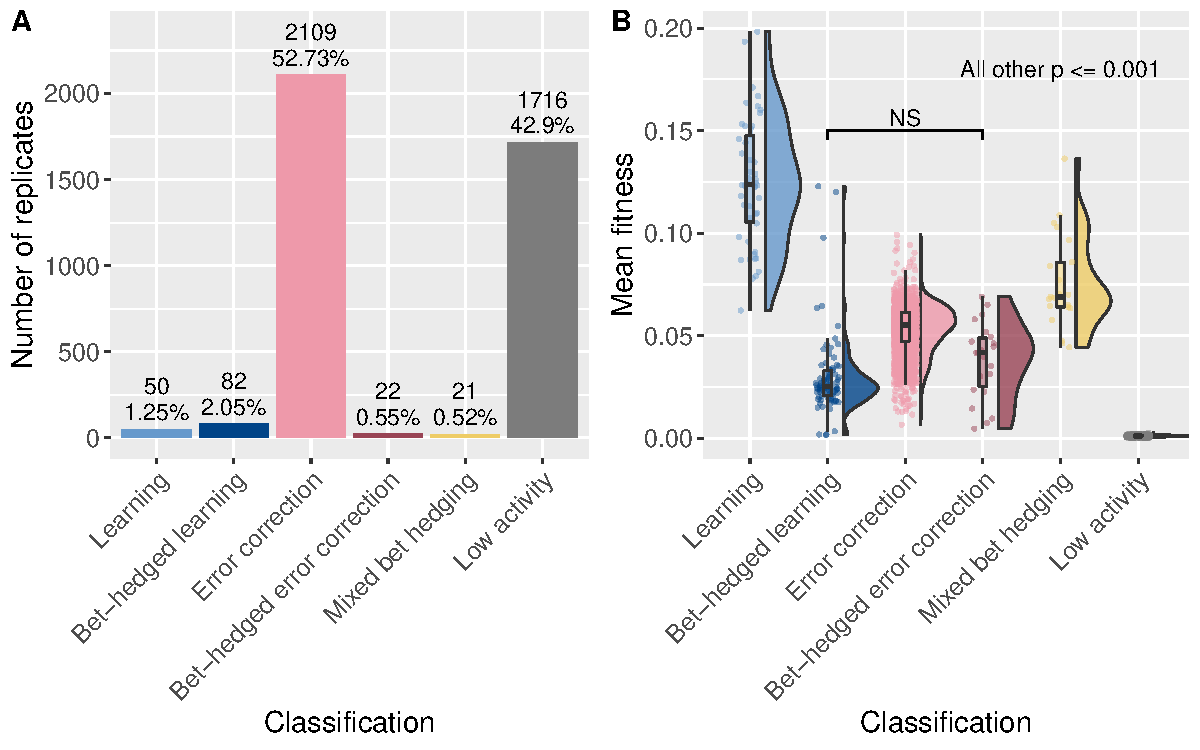
\includegraphics[width=0.9\textwidth]{04_learning_extension/media/initial_reps_stats.pdf}
\end{center}
\caption{ 
Subplot A) Columns show the number of initial replicates whose representative genotype evolved each type of behavior. 
Above each column, the numbers show the number of replicates that evolved that behavior and that count as a percentage of all 4,000 replicates. % (out of 4,000), while the bottom number shows the fraction of replicates.
Subplot B) Raincloud plots show fitness of all 4,000 initial replicates' representative genotypes, grouped by evolved behavior.
All pairwise comparisons are highly significant (p <= 0.001; Pairwise Mann-Whitney with Bonferroni correction) except for the one marked pair (bet-hedged learning and bet-hedged error correction did not have a significant difference).
}\label{fig:initial_reps}
\end{figure}


\subsection{The evolution of learning is exceedingly rare on random paths}
% Initial replicates (Outline)
    % Show categorical outcome figure
    % Learning DOES evolve, but only 1.25% of the time
    % Low activity and error correction account for >95% of replicates
    % Everything else is rare <= 3%
    % We can also look at fitness
        % We see that learning is the most efficient behavior
            % There is some overlap with learning-adjacent behavior (bet-hedged learning / mixed strategy bet-hedging)
        % Otherwise, error correction isn't too far behind learning (sig?)
    % Why is learning so rare here? 
            % It evolved in 8% of replicates in the other chapter
            % And even more than that in Anselmo's work
            % But here, we are evolving on *purely random paths*
            % This removes the first-cue guarantees, and creates a much more challenging bootstrapping problem

As shown in Figure \ref{fig:initial_reps}A, associative learning evolved in only 50 of 4,000 replicates (1.25\%). 
This is considerably lower than the probability of evolving associative learning in previous work, with 8\% of replicates evolving learning in Chapter \ref{chap:learning_case_studies} and up to 14\% in the ``two fixed turns'' environment of \citep{pontesEvolutionaryOriginAssociative2020}.
However, these higher success rates where observed in environments that guaranteed the order of one or more turns at the start of each path. 
In this work we have removed those guarantees entirely; the next step in the path is always uniformly chosen at random among a left turn, right turn, or a step straight ahead.
Thus, we must compare these results to the ``random start'' experiments in 
\citep{pontesEvolutionaryOriginAssociative2020}. 
In their work, zero of 50 replicates evolved learning under such conditions. 
This work therefore marks the first time that associative learning has evolved in Avida without any guarantees about cue ordering. 
It should be mentioned, however, that this work is more lenient with the \texttt{Move Backward} instruction, placing the organism directly back on the path instead of moving them one tile backward and requiring them to reorient on their own, as in \citep{pontesEvolutionaryOriginAssociative2020}.

While learning rarely evolved, error correcting behaviors evolved in the majority (53\%) of replicates. 
Similarly, most of the other replicates (43\%) were classified as ``Low Activity'' as, even at the end of the evolutionary replicate, they failed to correctly identify at least 25 cues in any of 100 trials. 
The remaining replicates evolved bet-hedged behaviors, with bet-hedged learning, bet-hedged error correction, and mixed bet hedging each present in less than 3\% of final evolved populations.

Finally, we see that organisms that perform learning have significantly higher fitness than organisms performing any other strategy (Figure \ref{fig:initial_reps}B, all $p << 0.001$, pairwise Mann Whitney with Bonferroni corrections for multiple comparisons). 
Mixed bet hedging has the next highest fitness, falling between its two constituent parts, learning and error correction. 
Bet-hedged learning and bet-hedged error correction both have lower fitness, on average, than their non-bet hedged counterparts. 
Finally, ``Low activity'' has very low fitness, as expected. 
These fitness values show us that learning was not rare because it was a poor solution to the problem, but rather due to the rugged nature of the underlying fitness landscape.

%\subsection{All replicates see windows of significant potentiation gain}
\subsection{Substantial increases in potentiation are common}

% Substantial increases in potentiation are common
    % We can look at this at two levels: 
        % 1. Exploratory (windows)
        % 2. Targeted (individual steps)
    % At the exploratory level *every* replayed replicate shows significant increase within a single window
        % This varies quite a bit, as we see in the distribution figures
    % At the targeted level, most replayed replicates show significant increase with a single step
        % But not all, we have exactly one non-significant replicate, and a few more are only weakly significant (p <= 0.05)
    % Is this consistent with preexisting replay replicates? 
        % In our work, yes!
        % Other digital studies?
            % Yedid? 
            % Covert?
        % In natural systems...
            % Zach's work... maybe?
            % Meyer paper?
            % C Turner paper? 
            % Jochmusen?
            % Other new papers?

\begin{figure}[h!]
\begin{center}
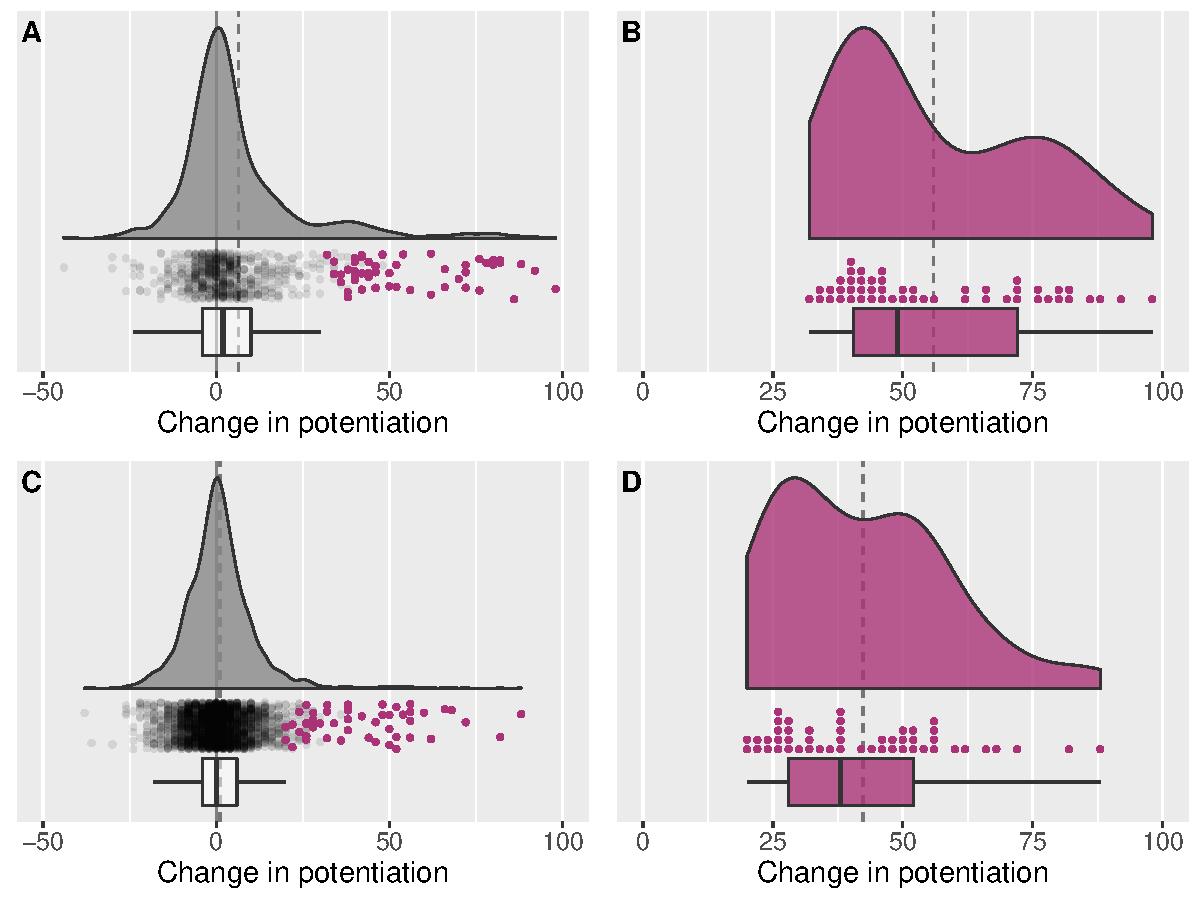
\includegraphics[width=0.9\textwidth]{04_learning_extension/media/replays_dists.pdf}
\end{center}
\caption{ 
Aggregate data for the exploratory replays (A,B) and targeted replays (C,D) of learning replicates. 
Subplots A and C) Raincloud plots showing the distribution of potentiation changes for the cumulative effects across all replayed windows (A) or the individual effects of all replayed lineage steps (C).
The solid vertical line shows zero change and the dashed vertical line shows the mean of the potentiation changes. 
For each of the 50 replicates, a purple point shows the maximum single-window (A) or single-step (C) potentiation increase.
These 50 points are then shown in isolation in (B) and (D).
Subplots B and D)  Raincloud plots showing the distribution of maximum single-window (B) or single-step (D) potentiation changes for each replicate (one point for each of the 50 learning replicates). 
The dashed vertical line shows the mean of these changes. 
}\label{fig:replay_distributions}
\end{figure}

\begin{figure}[h!]
\begin{center}
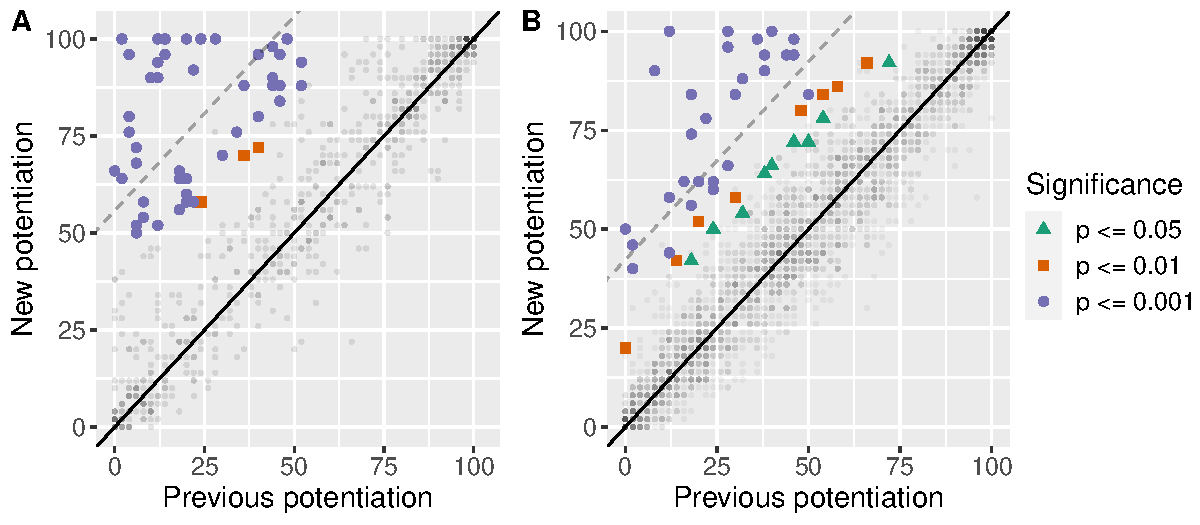
\includegraphics[width=0.9\textwidth]{04_learning_extension/media/replays_stats_legend_on_right.pdf}
\end{center}
\caption{ 
Scatter plot showing the potentiation before and after each exploratory window (Subplot A) or lineage step (Subplot B). 
The color and shape of the 50 main points show significance of the potentiation change (Fisher's exact test).
Semi-transparent points show the rest of the per-window (A, 10\% opacity) or per-step (B, 5\% opacity) potentiation changes. 
The line shows $y=x$, or no potentiation change. 
Potentiation gain is the vertical distance to this line. 
The dashed line shows the maximum potentiation gain of each replicate, averaged across all 50 replicates. 
}\label{fig:replay_stats}
\end{figure}

\begin{figure}[h!]
\begin{center}
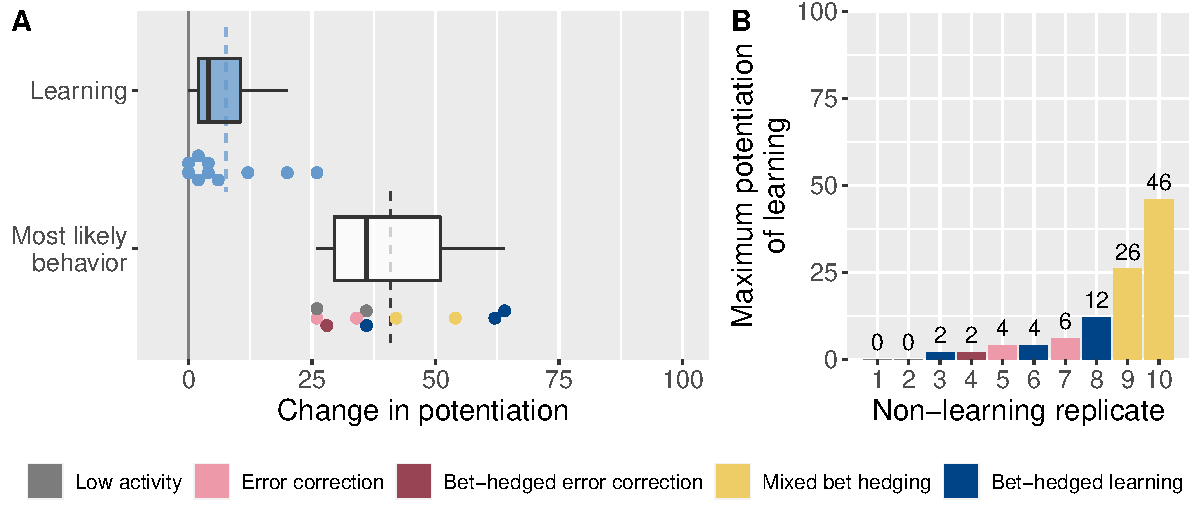
\includegraphics[width=0.9\textwidth]{04_learning_extension/media/non_learning_with_max.pdf}
\end{center}
\caption{ 
Subplot A) Distribution of the maximum per-window change in potentiation for learning (top) and most likely behavior to evolve (bottom) of each of the 10 replayed non-learning replicates.
Colors for the bottom distribution indicate the most likely behavior for each replicate.
Vertical dashed lines show the mean for each group.
Subplot B) The maximum potentiation level of learning observed in each of the 10 non-learning replicates, sorted. 
}\label{fig:non_learning}
\end{figure}

By number of replays conducted, this work is the largest study of potentiation via analytic replay experiments to date. 
Here we detail the key finding of this work: large increases in potentiation are not only possible, but are \textit{common} in this system.
This result is supported at multiple levels, as we detail below. 
For all 50 replicates, figures showing potentiation over time for both exploratory and targeted replays are available in the \hyperref[chap:app_a]{appendix}.

\subsubsection{All replicates have windows of significant potentiation gain}

Exploratory replays show us that, on average, the 50-step windows we replay show little potentiation gain (mean $\approx 6$, median = 2 percentage points) (see Figure \ref{fig:replay_distributions}A).
However, we see that these replays also cover a wide range, from -44 (i.e., 44 percentage points of potentiation \textit{loss)} to $+98$ (i.e., effectively full gain in potentiation in only 50 lineage steps). 

%When we consider the 50 learning replicates, we can also examine the maximum potentiation gain of each replicate (i.e., the potentiation gain of the \textit{potentiating window}).
When we consider these 50 learning replicates, we can also examine the maximum per-window potentiation gain of each replicate.
These maximum gains are highlighted in Figure \ref{fig:replay_distributions}A and shown in isolation in Figure \ref{fig:replay_distributions}B.
When only considering these maximum per-replicate gains, we see a mean gain of approximately $+56$, a median gain of $+49$, and a range of $[+32, +98]$ percentage points.
Figure \ref{fig:replay_stats}A shows all potentiation gains as a combination of their previous and new potentiation values. 
We see that potentiation increases significantly for all 50 learning replicates, even with only 50 replays each ($p \leq 0.01$, Fisher's exact). 
Indeed, 47 of these replicates are highly significant ($p \leq 0.001$). 
Thus we have further evidence that potentiation of learning can increase considerably in a relatively short amount of time. 

%\subsection{Large jumps in potentiation exist in most, but not all, replicates}
% \subsubsection{Large single-step increases in potentiation exist in most, but not all, replicates}
\subsubsection{Significant single-step increases in potentiation exist in all replicates}

While we see these large increases in potentiation over 50-step intervals, we can also look at smaller timescales. 
Indeed, the targeted, single-step replay results tell a similar story. 
Figure \ref{fig:replay_distributions}D shows the potentiation gains at \textit{all} replayed steps.
Here, the mean is approximately $+1$, the median is 0, and the range is $[-38, +88]$ percentage points. 
Thus we see a similar trend to the exploratory replays: the bulk of the distribution residing near zero, but with a short tail in the negative direction and a long tail in the positive direction. 

Focusing on only the maximum potentiating step for each lineage (Figure \ref{fig:replay_distributions}D), we see a mean of approximately $+42$, a median of $+38$, and a range of $[+20, +88]$ percentage points. 
Immediately we see that, in many replicates, a single step in the dominant lineage can account for 50 percentage points of the potentiation of associative learning. 
However, not all replicates see these huge jumps; multiple replicates have a potentiating step of less than 25 percentage points. 
When we examine the individual potentiating steps (Figure \ref{fig:replay_stats}B), we see that all of these changes are significant. 
Of the 50 replicates, 32 were significant at $p \leq 0.001$, nine more at $p \leq 0.01$, and the final nine additional replicates at $p \leq 0.05$. 

\subsubsection{Non-learning replicates see windows of potentiation increase in other behaviors}

We also see evidence of large gains in potentiation of behaviors other than learning. 
Figure \ref{fig:non_learning} details the results of our ten non-learning replicates that were replayed. 
Of these 10 replicates, the single-window potentiation gains for learning were relatively small, with a mean increase of $+7.6$, median of $+4$, and a range of $[0, +26]$ percentage points.
These low values are not surprising, however, as these lineages did not ultimately evolve learning. 
The potentiation for learning was never actualized and eventually lost. 
It should be noted that, even so, a potentiation gain of 26 percentage points over 50 lineage steps is substantial, which is highly significant ($p \leq 0.001$, Fisher's exact). 
Indeed, we see that one of the ten replicates reached a maximum learning potentiation of 46\% at one point in its evolutionary history, though seven replicates never crossed more than a 6\% chance of evolving learning (Figure \ref{fig:non_learning}B).

While the non-learning replicates did not see large increases in the potentiation of learning, they did see large increases in the potentiation of other behaviors. 
Figure \ref{fig:non_learning}A also shows the largest per-window potentiation increase in the most likely behavior at the end of evolution. 
Here we see a mean of $+40.8$, a median of $+36$, and a range of $[+26, +64]$ percentage points.
All of these differences are significant ($p \leq 0.01$, Fisher's exact), and eight of them highly significant ($p \leq 0.001$). 
Thus, the large increases in potentiation that we have observed are \textit{not} limited to the evolution of learning. 
% It should also be noted that two behaviors, error correction and low activity, are limited in their maximum potentiation gain. 
% Since both behaviors have a $>40\%$ chance of evolving from the naive ancestor (Figure \ref{fig:initial_reps}A), they either must first decrease in potentiation, or they are capped at $<60$ percentage points of gain in potentiation, and thus it is unlikely we would witness a 80 percentage point increase like we observed in the some learning replicates. 
Our expectation is that we would observe large single-step potentiation increases for these non-learning behaviors too if we conducted targeted replays on these lineages.
Figures of how potentiation changed over time for all 10 non-learning replicates are available in the \hyperref[chap:app_a]{appendix}. 
%appendix \ref{chap:app_a} (Figure \ref{fig:app_a_non_learning}).

\subsubsection{Comparison to other works}

In addition to a deeper investigation into the underlying patterN associated with historical contingency, the original motivation for this work was to validate the findings of Chapter \ref{chap:learning_case_studies} and provide evidence as to their generality. 
That is, we wanted to test if the large per-window and per-step increases we observed in that work were common or if they were mere flukes. 
Indeed, we can now confirm that both the per-window and single-step potentiation increases from that chapter are common in this particular system. 
The maximum per-step potentiation increases we observed in the previous chapter (range of $[+36, +64]$ percentage points) fall comfortably within the range that we observe here ($[+20, +88]$ percentage points).

% Our one direct comparison -- Blount et al. 2008
% Their jumps were much smaller
It is more difficult to compare these results to other works, however. 
While several works have leveraged replay experiments to study the potentiation of a particular trait or behavior, only one has applied replays to multiple points in a single lineage \citep{blountHistoricalContingencyEvolution2008}.
Blount et al. replayed multiple time points of frozen \textit{E. coli} from the Ara-3 strain to empirically test the potentiation of citrate metabolism. 
The largest jump in potentiation they found was \localapprox $+13.3\%$, shifting from $0/30$ replicates at generation 31,500 to $4/30$ replicates at generation 32,000 %(i.e., \localapprox 13.3 percentage points across 500 generations). 
This is a much smaller jump in potentiation, measured over a much longer period of time compared to our results in this work as the tests were 500 generations apart.

% Why might we be seeing larger increases in potentiation than in natural systems?
% There are a few (possibly confounding) factors:
% 1) The genetic landscape is much less complicated here than in natural organisms. 
% While Avida is much more complicated than many digital evolution systems, and in this particular system we have the possibility for many mutations from any given genotype (e.g., $>9000$ possible one-step mutations from a genome of length 100), this is nearly trivial in comparison to natural organisms. 
% This could mean that while there are many possible evolutionary paths in this system, there are still significantly fewer possibilities than in natural systems, and thus any individual paths is at a higher probability of selection. 
% 2) A lack of behavior-refinement needed in this system -- as discussed in \citep{blountGenomicAnalysisKey2012}, citrate metabolism underwent considerable refinement after it first evolved, and thus mutations to citrate metabolism might be lost to drift more frequently than learning-actualizing mutations in this system. 
% While associative learning in this system can be refined, we use an ``all or nothing'' definition and thus anything classified as learning should be relatively fit. 
% 3) E.coli evolved well over 100 million years ago, which should imply that they have settled into a rather stable region of the fitness landscape...


% The other good comparison -- Jochmusen et al 2016
While not directly pulling from an evolving lineage, \citet{jochumsenEvolutionAntimicrobialPeptide2016a} tested the effects of individual mutations on the evolution of colistin resistance in \textit{Pseudomonas aeruginosa}. 
Via experimental evolution, they found evidence that two individual mutations (\textit{phoQ} and \textit{pmrB}) each potentiated the evolution of colistin resistance at the $16\frac{\mu g}{ml}$ concentration level.
These two mutations each increased the potential to evolve this colistin level from  a $<5\%$ chance to a $>70\%$ chance. 
These results directly align with our results -- that a single mutation can drastically increase the probability of a focal behavior evolving. 

% Other works
% Caroline's work -- Never saw extinction in a replay
% Justin Meyer's work -- They were comparing across strains
% Art Covert's work -- Strong effect of a single deleterious mutation
% Dave Bryson's dissertation -- Strong effects in short term replays
For other works, \citet{turnerReplayingEvolutionTest2015} performed similar analytic replay techniques, but never saw the focal results -- the extinction of the Cit$^{-}$ clade in the Long Term Evolution Experiment -- in any of the replay replicates. 
\citet{meyerRepeatabilityContingencyEvolution2012} replayed combinations of Phage $\lambda$ and \textit{E. coli}. 
While some of their results are striking (e.g., the ``all-or-nothing`` pattern of OmpF receptor targeting across certain treatments), the comparisons were across strains and thus not a direct comparison. 
In prior digital work, \citet{covertiiiExperimentsRoleDeleterious2013} showed that a single deleterious mutation could increase the evolution of a complex behavior in Avida (the EQU logic task) from 13/20 (65\%) to 20/20 (100\%) of evolutionary replicates, providing further evidence of substantial potentiation gain from a single mutation.
Similarly, \citet{brysonEvolutionaryPotentialPopulations2012} showed multiple instances of $\geq 50$ percentage points of increase in short-term (always 10,000 updates) replays of EQU in Avida. 

% Do we want a paragraph summarizing these different results? 
% Most studies you cannot compare
% Those you can are mixed
%   A few have small changes (Blound, Turner)
%   Others match well (Jochmusen, Meyer, Covert III, Bryson)

\subsection{Increases in potentiation are often driven by a single mutation}
% Single mutations often drive increases in potentiation
    % Of our 50 replayed learning replicates, the largest potentiation step occured with only one mutation in 30 replicates
    % Of the 30 other replicates, we see that 14 of them have exactly one significant contributor, which is a standalone mutation

\begin{figure}[h!]
\begin{center}
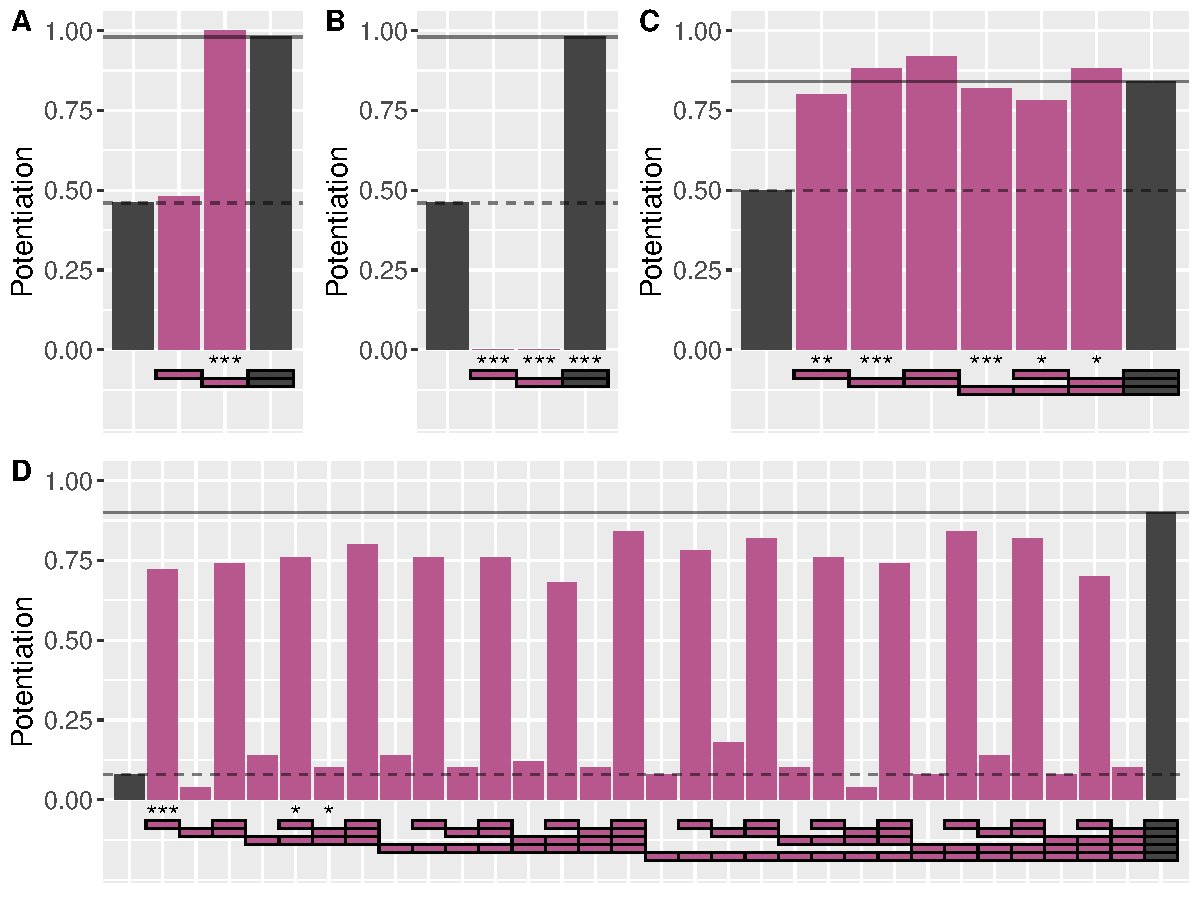
\includegraphics[width=0.9\textwidth]{04_learning_extension/media/mut_splits.pdf}
\end{center}
\caption{ 
Selected results from the mutation split experiment. 
For each subplot, the rightmost column shows the potentiation immediately after the largest potentiating step in that replicate (also shown via solid horizontal line), and the leftmost column shows the potentiation immediately before that step in the lineage (also shown via dashed horizontal line). 
This potentiating step involved $N$ mutations, where $N$ is 2 for subplots A and B, 3 for subplot C, and 5 for subplot D.
There are a total of $2^N$ bars in each subplot, representing the $2^N$ possible combinations of these mutations, as indicated by the small boxes below each bar.
The left bars show potentiation with none of the $N$ mutations presents, the right bars have all $N$ mutations present,
%These two steps are separated by $N$ mutations,
and the middle bars (purple) show the potentiation of every other possible combination of these mutations. 
Significance of each mutation combination in the logistic regression is shown under each column (* for $p \leq 0.05$, ** for $p \leq 0.01$, *** for $p \leq 0.001$). 
%Finally, the small boxes show the presence of individual mutations, with columns increasing in binary order.
In subplots A and D potentiation is driven by just one of the mutations; in B potentiation requires both mutations (which are individually lethal); and in C all three mutations are independently-potentiating. 
}\label{fig:mut_splits}
\end{figure}

For each of the learning lineages, we have identified the potentiating step; that is, the step in the phylogeny that conferred the largest increase in potentiation. 
Since Avida has a per-site rate for substitution mutations, and insertion and deletion mutations that can occur simultaneously, these lineage steps can consist of more than one mutation. 
Even so, 60\% of the potentiating steps (30 of 50) are comprised of only one mutation. 
Of the remaining 20 potentiating steps, 14 steps contained two mutations, three steps contained three mutations, one step contained four mutations, and two steps contained five mutations. 

Of course, the 30 potentiating steps that consisted of a single mutation must be driven by that particular mutation. 
For each of the other 20 potentiating steps (where multiple mutations co-occurred), we ran replay experiments to split the mutations and determined that not all were necessary to increase potentiation. 
Indeed, % of the 20 steps that consisted of more than one mutation, 
in 14 cases we identified exactly one mutation that significantly increased potentiation on its own. 
The two steps involving five-mutation are included here, as a single mutation explained the potentiation gain in both cases. 
Data from an example of potentiation being driven by one of two co-occurring mutations can be seen in Figure \ref{fig:mut_splits}A, and an example of one driving mutation out of five total mutations can be seen in Figure \ref{fig:mut_splits}D. 

As discussed above, other work has shown that single mutations can have a large impact on potentiation. 
This has been shown in colistin resistance in \textit{Pseudomonas aeruginosa} \citep{jochumsenEvolutionAntimicrobialPeptide2016a} and in the evolution of EQU in Avida \citep{covertiiiExperimentsRoleDeleterious2013}.
Thus we have instances where potentiation increases drastically with single mutations in both digital and natural organisms. 
% Conversely, while we see some evidence for the slow accumulation of potentiation (i.e, 50-step windows with significant potentiation gain but no individual mutations within the window that significantly increase potentiation), we have not found evidence of this dynamic in natural systems in the potentiation literature. 


\subsection{Mutation interactions influence potentiation}
% Mutation interactions influence potentiation
    % Of the 6 replicates that did not rely on one single mutation, at least four had interesting interactions among there mutations
    % Two had epistatic interactions -- the individual mutations were lethal, but together they were potentiating
    % One had two mutations additively accounting for the increase in potnetiation
    % One had three independent mutations, where each mutation would have increased potentiation, but the combination did nothing
    % The final two had no significant factors, and thus we cannot classify them


While we are able to confidently say that many replicates saw potentiation increase with a single mutation, we also observed instances where potentiation changes appeared to require interactions across multiple simultaneous mutations, or other unexpected interactions. %, including their interactions, can influence potentiation.
We identified one replicate where two mutations independently increased potentiation, and combined they accounted for the full step's potentiation gain. 
In one of the steps containing three mutations, all three mutations independently increased potentiation significantly, but the combination of mutations did not further increase potentiation (Figure \ref{fig:mut_splits}C). 
In two replicates we see strong sign epistasis; each step consisted of two mutations, and when analyzed independently these mutations proved to be lethal (and thus potentiation is 0), but when the mutations were combined the resulting mutants were not only viable, but potentiated (Figure \ref{fig:mut_splits}B). 
This is akin to the case study of EQU potentiation in \citep{covertiiiExperimentsRoleDeleterious2013}, where two deleterious mutations (one nearly lethal) combined to actualize EQU.
Finally, of the 50 replicates, two were found to have no significant mutation effects, and further replicates would be required to disentangle the effects of the mutations and their interactions.

%\subsection{Potentiating mutations are still undetectable as they occur in an evolving population}
%\subsection{Potentiating mutations are cryptic in evolving populations}
\subsection{No real-time hallmarks of potentiating mutations were evident in an evolving population}

\begin{figure}[h!]
\begin{center}
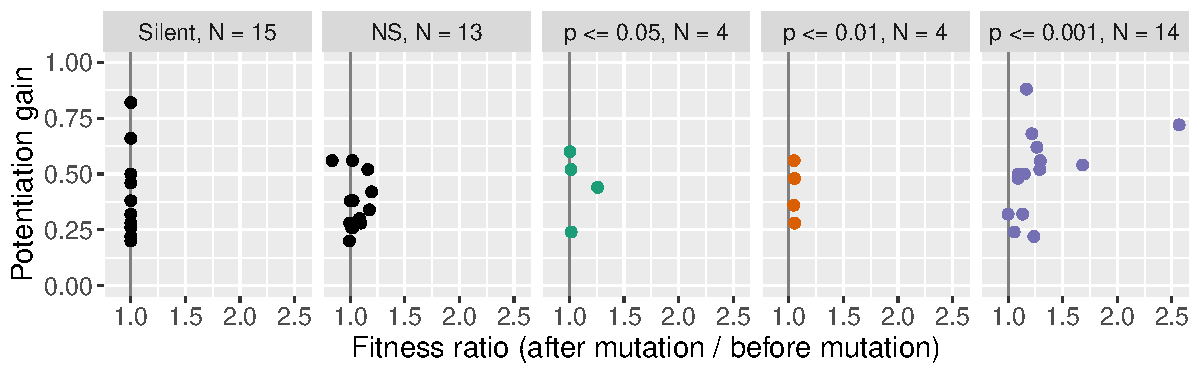
\includegraphics[width=0.9\textwidth]{04_learning_extension/media/fitness_diffs.pdf}
\end{center}
\caption{ 
The fitness effect and potentiation gain of the potentiating step of all 50 learning replicates. 
To calculate fitness, both the potentiation step and the step before it were evaluated on the same set of 100 random seeds. 
We ran a paired Wilcoxon rank-sum test for these two fitness groups for each replicate, and divided and colored the results based on these significance findings. 
Non-significant points are split into those that are truly silent mutations (i.e., zero change in fitness across all 100 trials) and those that are not (fitness values changed, but not significantly). 
The fitness ratio, used for the x-axis, is calculated as the average post-mutation fitness divided by the average pre-mutation fitness. 
The vertical line shows a fitness ratio of one, which indicates no change in the average effect. 
}\label{fig:fitness_diffs}
\end{figure}

As discussed in Chapter \ref{chap:learning_case_studies}, while we can retrospectively identify potentiating mutations, we have yet to find strong indicators of these mutations \textit{during evolution}.
Any such consistent indicators would be invaluable for problem solving with evolutionary computation or other forms of applied evolution. 

Our early hypothesis was that these potentiating mutations are likely to be deleterious, or at least neutral. 
Our reasoning was that if the mutations are beneficial, they would already be likely to be selected and thus they would already be factored into  %expect that their appearance would not drastically alter long-term 
evolutionary potential. 
Of the four case study lineages in Chapter \ref{chap:learning_case_studies}, we saw that one potentiating step was deleterious, two were neutral, and one was beneficial. 

Here, we have refined our methods to compare the potentiating step to the step before it, evaluating both genotypes on the same set of 100 random paths to conduct a pairwise comparison (Figure \ref{fig:fitness_diffs}). 
Using a paired Wilcoxon test, we find that in 28 of 50 lineages the potentiating step did not have a significant effect on realized fitness. 
Indeed, in 15 of these replicates, the two genotypes displayed \textit{exactly} the same behavior -- the mutations were truly silent, while in 13 changes to fitness occurred, but not enough to meaningfully change the distribution.
The truly neutral mutations may be modifying instructions that are executed but do not directly effect the phenotype, or they could be cryptic genetic variation occurring in unexpressed regions of the genotype (Chapter \ref{chap:consequences_of_plasticity}). 
Of the remaining 22 replicates with significant changes to fitness, we find that 21 significantly increase fitness, and only one mutation was significantly deleterious. 
Further, our one deleterious mutation was significant ($p < 0.001$) but not substantial, with less than a 1\% change in fitness. 

The fitness effects of the significantly beneficial mutations varied wildly,  with many conferring small impacts on fitness. 
Two mutations had a greater than 50\% increase in fitness, one of which had a fitness over 250\% of the pre-mutation fitness. 
Thus, we have strong evidence against our hypothesis that potentiating mutations are likely deleterious. 
We observe that potentiating mutations are often neutral or nearly-neutral, though they can also drastically increase fitness. 
%In a genetic space as complicated as Avida's, we now realize that even if a mutation is highly beneficial, there are likely other highly-beneficial mutations, even if they are few, and thus these beneficial mutations are not guaranteed to sweep and thus can affect potentiation.
In a genetic space as complicated as Avida's, even highly-beneficial mutations are not guaranteed to be found, let alone sweep.
Given the number of alternative possibilities, some of which may be highly advantageous themselves, even beneficial mutations can be highly potentiating.
Indeed, even if deleterious mutations would open up new pathways through the genotype space, the low probability of them gaining substantial numbers in the population may eliminate the possibility of them being potentiating.

One final hypothesis for identifying potentiation mutations \textit{as they occur} is to look for mutations that alter the overall behavioral phenotype. 
Of the 50 potentiating lineage steps that we analyzed, we found that 43 of 50 left the underlying behavioral phenotype unchanged. 
Of the seven that did change the phenotype, all were originally error correction behaviors. 
After the potentiating step, five then shifted to a mixed bet hedging strategy -- they still performed error correction on some paths but were capable of learning on others. 
One more replicate evolved learning \textit{with the potentiating step}, likely representing a low probability mutation that was actualized. 
The final behavior-changing mutation shifted the behavior from error correction to bet-hedged error correction. 
While this replicate might represent an interesting case -- the degradation of behavior -- the majority of potentiating mutations did not change the behavior and thus behavior changes are not a reliable indicator of potentiating mutations when they occur. 
%% Discussion
% This section may be divided by subheadings. Discussions should cover the key findings of the study: discuss any prior research related to the subject to place the novelty of the discovery in the appropriate context, discuss the potential shortcomings and limitations on their interpretations, discuss their integration into the current understanding of the problem and how this advances the current views, speculate on the future direction of the research, and freely postulate theories that could be tested in the future.

\section{Discussion}
% Discussion outline
    % Large single-step potentiation gains are common, but not ubiquitous
        % Median > 35%, Mean > 40%
        % Some jumps are as large as 80%
        % However, we also see instances as low as 20%
        % How many are significiant?

    % These potentiating events are overwhelmingly driven by single mutations
        % 30/50 were just one mutation to start with, 14 more seem to be driven by one mutation 

    % Still no metrics to detect potentiating mutations as they occur
        % Fitness effects can be anything
        % Only a few (7/50) change the behavioral phenotype
Here we place the results of this work in a broader evolutionary biology context. 

\subsection{Drastic increases in potentiation are common}

\subsection{Single mutations often drive increases in potentiation}

\subsection{Mutation interactions influence potentiation}

\subsection{Potentiating mutations are still undetectable in an evolving population}

\section{Conclusion}
% Conclusion (outline)
    % This is the first study to look into potentiation in the aggregate
        % How does this relate to other studies? 
            % Confirms ALife 2023 was not a fluke
            % Provides evidence of step-function potentiation (a la Blount 2008)
            % Other papers? 
    % Is this applicable to natural systems? 
        % Not directly!
        % The methods could be employed, but this does not mean that this effect is seen in other digital systems, let alone in natural systems. 
    % Future work
        % Expand to other systems

% General intro - what have we done here?
Here we have conducted a study of potentiation with the largest number of analytic replay experiments to date.
By replaying 50 lineages of digital organisms that evolved associative learning, we have provided further evidence that potentiation can increase suddenly, with strong evidence that a single mutation can result in large increases in potentiation. 
We have also shown that potentiation can increase as a result of the co-occurrence of multiple mutations, with or without epistatic interactions. 
Finally, we were unable to find a signal for these potentiating mutations when they appear -- as such, we are still only able to identify these mutations retrospectively. 

\subsection{Limitations and applicability to other systems}
% This system is clearly digital

% We see similar dynamics in some works in natural systems

% However, some works saw much smaller increases in potentiation
% Factors: 
%   - Simpler genetic landscape
%   - Learning is very likely to stick around
%       - In part because it requires very little refinement to be beneficial

% Using clonal population restarts will create larger jumps in potentiation than population snapshots

%

In both this work and Chapter \ref{chap:learning_case_studies} we primarily investigate the potentiation of one behavior, associative learning, in the Avida digital evolution framework. 
As such, we cannot claim that the potentiation dynamics observed in this work are globally applicable. 
Indeed, we can only claim these results as evidence that large, single-mutation increases in potentiation are \textit{possible}, and that, in certain systems, they might be common. 

While this work is among the first to explore \textit{patterns} in potentiation across many evolved lineages, it is far from the first to explore potentiation dynamics. 
Do the results of other studies match the large increases in potentiation we observed for the evolution of associated learning in Avida? 
In some cases it appears that short spans of evolution, and in fact even single mutations, confer substantial increases in potentiation \citep{jochumsenEvolutionAntimicrobialPeptide2016a, covertiiiExperimentsRoleDeleterious2013}. 
These increases are not universal, as other works have seen maximum increases in potentiation substantially lower than observed here \citep{blountHistoricalContingencyEvolution2008}.
In conducting these comparisons, however, we must consider that the sample sizes for these other works are quite low and that may bias our comparisons.
Additionally, all replay replicates in \citep{blountHistoricalContingencyEvolution2008} evolved for the same number of generations regardless of the starting point, while we ensured that all replay replicates experienced the same number of Avida updates as the original lineage experienced after the sampled genotype appeared. 
We would expect the former scheme to observe substantially lower potentiation in replicates founded from earlier points in the population's history. 
Finally, it is possible that the lineages in these other studies \textit{did} see substantial increases in potentiation, but those particular changes were missed in those experiments. 

% Our mutational neighborhoods are smaller, and thus any given mutation is more likely to occur
If these potentiation dynamics truly differ, what might explain these differences? 
While Avida has a rich and complex genetic architecture compared to many other digital evolution experiments, these digital organisms are still vastly less complex than even the most simple natural bacteria.
An Avida organism in this work, with our original genome length of 100 instructions, has roughly 9,000 possible one-step mutations that can occur. 
With a naive assumption that every nucleotide could mutate to any other nucleotide at every site in the \textit{E. coli} genome (\localapprox 4.6 million base pairs, \citet{blattner1997complete}), we would expect over 13 million one-step substitution mutations alone. 
While this is only a rough estimate, it is clear that the likelihood of a particular mutation appearing is much lower in natural organisms, which can bias the potentiation changes. 
This difference only compounds as we consider the likelihood of multiple necessary mutations arising and fixing.
Therefore, we expect that natural organisms will typically see lower levels of potentiation for equivalent genetic distances from the focal behavior.

% Learning in our system needs little refinement, and also it is a "terminal" behavior
Additionally, there is likely a difference in how the focal behavior arises and is classified. 
We are stringent in our system and only classify a behavior as learning if it is already well-refined, and thus even the first organism in the population to be classified as having evolved learning is likely to have high fitness. 
In natural systems, biologists will often denote a non-trivial trait or behavior as present even if it still requires considerable refinement. 
For example, in the \textit{E. coli} studies in the LTEE, citrate metabolism was not highly advantageous initially, but rather needed considerable refinement before it rose to prominence in the population \citep{blountGenomicAnalysisKey2012}.
Thus, even genotypes capable of weak citrate metabolism may still have low potentiation for maintaining that trait in the longer term, as it may be lost before it is refined. 
Follow-up work to our study should consider analyzing the potentiation of all forms of learning, including bet-hedged learning and mixed bet hedging strategies that combine learning and error correction, to see if potentiation dynamics change. 
Further, learning is a terminal behavior in our system -- the lack of open-endedness dictates that once learning evolves, it is unlikely to be replaced with a more effective survival strategy. 
Combined, these factors may create larger increases in potentiation, and should be dissected in future digital studies. 

% Final, clonal populations vs population snapshots, population sizes
Finally, our system uses small population sizes (3,600 organisms) compared to natural systems (which are often in excess of tens of millions of organisms), and our replay techniques may also bias the changes in potentiation. 
By using a smaller population size, we increase the effect of genetic drift on our population and increase the likelihood that neutral or even deleterious mutations can spread before being purified. 
In fact, by replaying populations via a full clonal population of an genotype from the dominant lineage, we are resetting all population dynamics from the potentiation measurements. 
During normal evolution of a population, not only does a mutation need to occur, but the organism in which it resides also needs to successfully replicate at least once. 
By using clonal populations for our replay experiments, we ensure that every mutation establishes, eliminating possible intermediate potentiation values. 

\subsection{Future work}

% Other analyses?
    % Distance to focal behavior
        % Meaningful distance to focal behavior
    % Did the potentiating mutation exist at the time of actualization

% Expanding beyond Avida and learning
In this chapter we described our deep analysis of the potentiation dynamics behind the evolution of associative learning in Avida. 
First and foremost, future work should investigate potentiation dynamics in a range of other systems. 
Digital systems as simple as bitstring evolution problems could illuminate how the dynamics are affected by factors such as mutation rate and population size. 
Slightly more complicated systems could investigate characteristics of the genetic space such as connectedness, dimensionality, mutational operators, or crossover.
Finally, more wet-lab studies of potentiation across a wider range of environments or in a more varied selection of natural organisms can provide more real-world grounding for these results, though such systems are considerably more labor-intensive. 

% Other potentiation dynamics - anti-potentiating mutations
As we alluded to in Chapter \ref{chap:learning_case_studies}, not only are we interested in identifying mutations that substantially increase potentiation, but we are also interested in the mutations that significantly \textit{decrease} potentiation. 
In this work we replayed ten replicates that did not evolve associative learning, to see how their potentiation dynamics differed from ``successful'' replicates. 
Even within those ten replicates we observed one replicate that reached a height of 46\% potentiation for associative learning. 
Extending this idea, if we have 50 replicates that evolved learning, we might expect 100 replicates to have reached 50\% potentiation but only half of them to have succeeded in that coin flip. 
This conjures the question: do we see large decreases in potentiation similar to the increases observed in this work? 
Are there single mutations that doom a would-be promising lineage to an ``unsuccessful'' fate? 
For example, an immediately beneficial mutation might sweep through a population trapping it on a local optima and preventing it from following a pathway that would lead a population to higher levels of fitness.
Identifying these anti-potentiating mutations in real time could potentially be as valuable as identifying potentiating mutations as they could allow us to slow the evolution of pathogenic or otherwise harmful populations.
While additional studies would be needed to fully delve into these dynamics, early work should dive into this dataset. 
When conducting replay experiments, we are effectively quantifying the potentiation of \textit{each} possible behavior. 
Thus we have non-learning potentiation data, but analyzing this data is outside the scope of this chapter. 

% Improving methods
Finally, additional work is needed to identify techniques that reduce the cost of performing replay experiments. 
This work has taken one step: iterating backward from the appearance of the focal behavior during the exploratory replay phase. 
Additional optimizations could include minimizing the original number of replicates per replayed time step and then running additional replicates for those that seem interesting. 
Finding more efficient ways of searching for potentiating steps is critical. 
We cannot directly perform a binary search for finding the largest potentiating step, as potentiation does not increase monotonically and thus large increases in potentiation can be hidden by decreases in the same window. 
However, there may be variations of binary search that will provide the maximum potentiating step within some margin of error or the maximum \textit{sustained} increase in potentiation. 
In particular, using digital systems to find and verify these ideas might make future \textit{in vitro} experiments more tractable to perform. 

% Conclusion
Overall, these results provide a useful benchmark for any future projects that use replay experiments to study historical contingency. 
As more studies of mutations are conducted, we can refine our ideas about how potentiation changes over the course of a population's history. 
As we progress, we can leverage our understanding of potentiation dynamics to better infer what happened in the evolution of life around us, better prepare for how populations will evolve under climate change, and better leverage evolution to solve technical problems. 